
We demonstrate the effectiveness of the ACD self-supervision across a range of experimental scenarios. 
For all the experiments in this section we use ACDs computed on all shapes from the ShapeNetCore data~\cite{Chang2015ShapeNetAI},
which contains 57,447 shapes across 55 categories.
The decomposition was computed using a concavity tolerance of $1.5 \times 10^{-3}$ and a volumetric
grid of resolution $128^3$.
All the other parameters are set to their default values according to a 
publicly available implementation\footnote{\url{https://github.com/kmammou/v-hacd}} of~\cite{vhacd}.
The resulting decompositions have an average of 17 parts per shape.


% ============================================================
\subsection{Shape classification on ModelNet}
In this set of experiments, we show that the representations learned by a network trained on ACD are useful for discriminative downstream tasks such as classifying point clouds into shape categories. 


% ------------------------------------------------------------
%\begin{figure}[t]
%    \centering
%    \includegraphics[width=\linewidth]{imgs/featvis.pdf}
%    % \framebox(\textwidth,90pt){}
%    \caption{A couple of these feature are wrong (global instead of local) \todo Fix this.}
%    \label{fig:my_label}
%\end{figure}


\vspace{2mm}
\noindent
\textbf{Dataset.} We report results on the ModelNet40 shape classification benchmark, which consists of 12,311 shapes from 40 shape categories in a train/test split of 9,843/2,468. A linear SVM is trained on the features extracted on the training set of ModelNet40. 
%We created a validation set from 20\% of the training samples of ModelNet40 to find the optimal setting of $C$ for the SVM. 
This setup mirrors other approaches for unsupervised learning on point clouds, such as FoldingNet~\cite{yang2018foldingnet} and Hassani~\etal~\cite{hassani2019unsupervised}.

\vspace{2mm}
\noindent
\textbf{Experimental setup.} 
A PointNet++ network is trained on the unlabeled ShapeNet-Core data using the pairwise contrastive loss on the ACD task, using the Adam optimizer, initial learning rate of 1e-3 and halving the learning rate every epoch. 
However, this network architecture creates an embedding for each of the $N$ points in an input shape, 
while for the shape classification task we require a single global descriptor for the entire point cloud.
%\rui{this sentence is confusing, should rephrase}. 
Therefore, we aggregate the per-point features of PointNet++ at the first two set aggregation layers (\texttt{SA1} and \texttt{SA2}) and the last fully connected layer (\texttt{fc}), resulting in 128, 256 and 128 dimensional feature vectors, respectively. Since features from different layers may have different scales, we normalize each vector to unit length before concatenating them, and apply element-wise signed square-rooting~\cite{sanchez2013image}, resulting in a final 512-dim descriptor for each point cloud.
The results are presented in Table~\ref{tab:modelnet}.
 
\vspace{2mm}
\noindent
\textbf{Comparison with baselines.}
As an initial na\"ive baseline, we use a PointNet++ network with random weights as our feature extractor, 
and then perform the usual SVM training. 
This gives 78\% accuracy on ModelNet40 -- while surprisingly good, the performance is not entirely unexpected: 
randomly initialized convolutional neural networks are known to provide useful features by virtue of their architecture, 
as studied in Saxe~\etal~\cite{saxe2011random}. 
Training this network with ACD, on the other hand, gives a significant boost to performance (78\% $\rightarrow$ \textbf{89.1}\%), 
demonstrating the effectiveness of our proposed self-supervision task. 
This indicates some degree of generalization across datasets and tasks -- from distinguishing convex components on ShapeNet to classifying shapes on ModelNet40.
Inspired by~\cite{hassani2019unsupervised}, we also investigated if adding a reconstruction component to the loss
would further improve accuracy.
Reconstruction is done by simply adding an AtlasNet~\cite{atlasnet} decoder to our model and using Chamfer distance
as reconstruction loss.
Without the reconstruction term (i.e. trained only to perform ACD using contrastive loss), our result accuracy ($89.1\%$) is the same as the multi-task learning approach presented in~\cite{hassani2019unsupervised}.
After adding a reconstruction term, we achieve an improved accuracy of  $\mathbf{89.8\%}$.
On the other hand, having just reconstruction without ACD yields an accuracy of $86.2\%$.
This shows not only that ACD is a useful task when learning representations for shape classification, but that it can also be combined
with shape reconstruction to yield even better results.

\vspace{2mm}
\noindent
\textbf{Comparison with previous work.} 
Approaches for \textit{unsupervised} or \textit{self-supervised} learning on point clouds are listed in the upper portion of Table~\ref{tab:modelnet}. Our method achieves \textbf{89.1\%} classification accuracy from purely using the ACD loss, which is met only by the unsupervised multi-task learning method of Hassani~\etal~\cite{hassani2019unsupervised}. We note that our method merely adds a contrastive loss to a standard architecture (PointNet++), without requiring a custom architecture and multiple pretext tasks as in \cite{hassani2019unsupervised}, which uses clustering, pseudo-labeling and reconstruction.


% ------------------------------------------------------------
\begin{table}[t]
\centering
\caption{\small{Unsupervised shape classification on the ModelNet40 dataset.
%\rui{should clarify what are the groups of methods being compared here: unsupervised or self-supervised}. 
The representations learned in the intermediate layers by a network trained for the ACD task on ShapeNet data are general enough to be useful for discriminating between shape categories on ModelNet40. 
% ($*$~\cite{sauder2019self} selects the best model w.r.t. ModelNet40 performance, unlike others which are fully unsupervised and do not use the downstream task for model selection).
}}
\label{tab:modelnet}
\begin{tabular}{@{\extracolsep{5pt}}lc}
\toprule
 \textbf{Method}                           & \textbf{Accuracy (\%)}  \\
\midrule 
  VConv-DAE~\cite{sharma2016vconv}         & 75.5    \\
  3D-GAN~\cite{wu2016learning}            & 83.3    \\
  Latent-GAN~\cite{achlioptas2017representation}        & 85.7    \\
  MRTNet~\cite{mrt18}                                   & 86.4 \\
  PointFlow~\cite{yang2019pointflow}                    & 86.8 \\
  FoldingNet~\cite{yang2018foldingnet}        & 88.4   \\
  PointCapsNet~\cite{zhao20193d}              & 88.9 \\
  Multi-task~\cite{hassani2019unsupervised}   & 89.1 \\
\midrule
  Our baseline (with Random weights)           & 78.0 \\
  With reconstruction term only          & 86.2 \\
%   PointNet++ random wts            & 77.96 \\
%   PointNet++ ACD                   & 86.71 \\
%   PointNet++ ACD w/ z-rot          & 88.17 \\
%   PointNet++ ACD w/ z-rot, sqrt    & \textbf{89.06} \\
  Ours with ACD    & 89.1 \\
  Ours with ACD + Reconstruction    & \textbf{89.8} \\
% ACD-\textit{dict}    & \textbf{...} \\
\bottomrule
\end{tabular}
\end{table}


% \noindent
% \textbf{On learning ACD and classification performance.} 
% \todo



% ============================================================
\subsection{Few-shot segmentation on ShapeNet}

\noindent
\textbf{Dataset.} We report results on the \textbf{ShapeNetSeg} part segmentation benchmark~\cite{Chang2015ShapeNetAI}, which is a subset of the ShapeNetCore database with manual annotations (train/val/test splits of 12,149/1,858/2,874). It consists of 16 man-made shape categories such as airplanes, chairs, and tables, with manually labeled semantic parts (50 in total), such as wings, tails, and engines for airplanes; legs, backs, and seats for chairs, and so on. Given a point cloud at test time, the goal is to assign each point its correct part label out of the 50 possible parts.  Few-shot learning tasks are typically described in terms of ``$n$-way $k$-shot'' -- the task is to discriminate among $n$ classes and $k$ samples per class are provided as training data. We modify this approach to our setup as follows -- we select $k$ samples from each of the $n=16$ shape categories as the labeled training data, while the task remains semantic part labeling over the 50 part categories.

% ------------------------------------------------------------
\begin{table}[t]
\centering
\caption{\small{Few-shot segmentation on the ShapeNet dataset (\textit{class avg. IoU} over 5 rounds). $K$ denotes the number of shots or samples per class for each of the 16 ShapeNet categories used for supervised training. Jointly training with the ACD task reduces overfitting when labeled data is scarce, leading to significantly better performance over a purely supervised baseline.
}}
\label{tab:shapenet}
\begin{tabular}{@{\extracolsep{5pt}}lcccc}
\toprule
Samples/cls.    & \textbf{k=1}      & \textbf{k=3}      & \textbf{k=5}     & \textbf{k=10}   \\
\midrule 
  Baseline      & 53.15 $\pm$ 2.49  & 59.54 $\pm$ 1.49  & 68.14 $\pm$ 0.90 & 71.32 $\pm$ 0.52  \\
  w/ ACD        & 61.52 $\pm$ 2.19  & 69.33 $\pm$ 2.85  & 72.30 $\pm$ 1.80 & 74.12 $\pm$ 1.17  \\
\toprule
                & \textbf{k=20}     & \textbf{k=50}      & \textbf{k=100}      & \textbf{k=inf}   \\
\midrule
  Baseline      & 75.22 $\pm$ 0.82  &  78.79 $\pm$ 0.44  &  79.67 $\pm$ 0.33   & 81.40 $\pm$ 0.44  \\
  w/ ACD        & 76.19 $\pm$ 1.18  &  78.67 $\pm$ 0.72  &  78.76 $\pm$ 0.61   & 81.57 $\pm$ 0.68  \\
  
\bottomrule
\end{tabular}
\end{table}


\noindent
\textbf{Experimental setup.} 
 For this task, we perform \textit{joint training} with two losses -- the usual cross-entropy loss over labeled parts for the training samples from ShapeNetSeg, and an additional contrastive loss over the ACD components for the samples from ShapeNetCore (Eq.~\ref{eq:joint}), setting $\lambda = 10$. In our initial experiments, we found joint training to be more helpful than pre-training on ACD and then fine-tuning on the few-shot task (an empirical phenomenon also noted in \cite{xie2019self}), and thereafter consistently used joint training for the few-shot experiments. All overlapping point clouds between the human-annotated ShapeNetSeg and the unlabeled ShapeNetCore were removed from the self-supervised training set. The $(x, y, z)$ coordinates of the points in each point cloud are used an the input to the neural network; we do not include any additional information such as normals or category labels in these experiments.


\vspace{2mm}
\noindent
\textbf{Comparison with baselines.}  Table~\ref{tab:shapenet} shows the few-shot segmentation performance of our method, versus a fully-supervised baseline. 
Especially in the cases of very few labeled training samples ($k=1, \dots, 10$), 
having the ACD loss over a large unlabeled dataset provides a consistent and significant gain 
in performance over purely training on the labeled samples. 
As larger amounts of labeled training samples are made available, 
naturally there is limited benefit from the additional self-supervised loss -- 
\eg when using all the labeled data, our method is within standard deviation of the purely supervised baseline.
Qualitative results are shown in Fig.~\ref{fig:segresults}.

\vspace{2mm}
\noindent
\textbf{Comparison with previous work.}
The performance of recent \textit{unsupervised} and \textit{self-supervised} methods on ShapeNet segmentation are listed in Table~\ref{tab:sota_shapenet}. Consistent with the protocol followed by the multi-task learning approach of Hassani~\etal~\cite{hassani2019unsupervised}, we provide 1\% and 5\% of the training samples of ShapeNetSeg as the labeled data and report instance-average IoU. Our method clearly outperforms the state-of-the-art unsupervised learning approaches, improving over \cite{hassani2019unsupervised} at both the 1\% and 5\% settings (68.2 $\rightarrow$ \textbf{75.7}\% and 77.7 $\rightarrow$ \textbf{79.7}\%, respectively). 

% ------------------------------------------------------------
\begin{table}[t]
\centering
\caption{\small{Comparison with state-of-the-art semi-supervised part segmentation methods on ShapeNet. Performance is evaluated using \textit{instance-averaged IoU}.
}}
\label{tab:sota_shapenet}
\begin{tabular}{@{\extracolsep{5pt}}lcc}
\toprule
 \multirow{2}{*}{\textbf{Method}}                          &  1\%~labeled         &  5\%~labeled \\
                                          & \textbf{IoU}         & \textbf{IoU} \\
\midrule 
 SO-Net~\cite{li2018so}                    &  64.0               & 69.0 \\
 PointCapsNet~\cite{zhao20193d}            &  67.0               & 70.0 \\
 MortonNet~\cite{MortonNet}               &  -               & 77.1 \\
 Multi-task~\cite{hassani2019unsupervised} &  68.2               & 77.7 \\
\midrule
 ACD (\textit{ours})                       &  {\bf 75.7}    &  {\bf 79.7} \\ 
                                        %   &   $\pm$ 0.48  &  $\pm$ 1.75    &   ....  & ... \\
\bottomrule
\end{tabular}
\end{table}



% ------------------------------------------------------------
\begin{figure}[t]
    \centering
    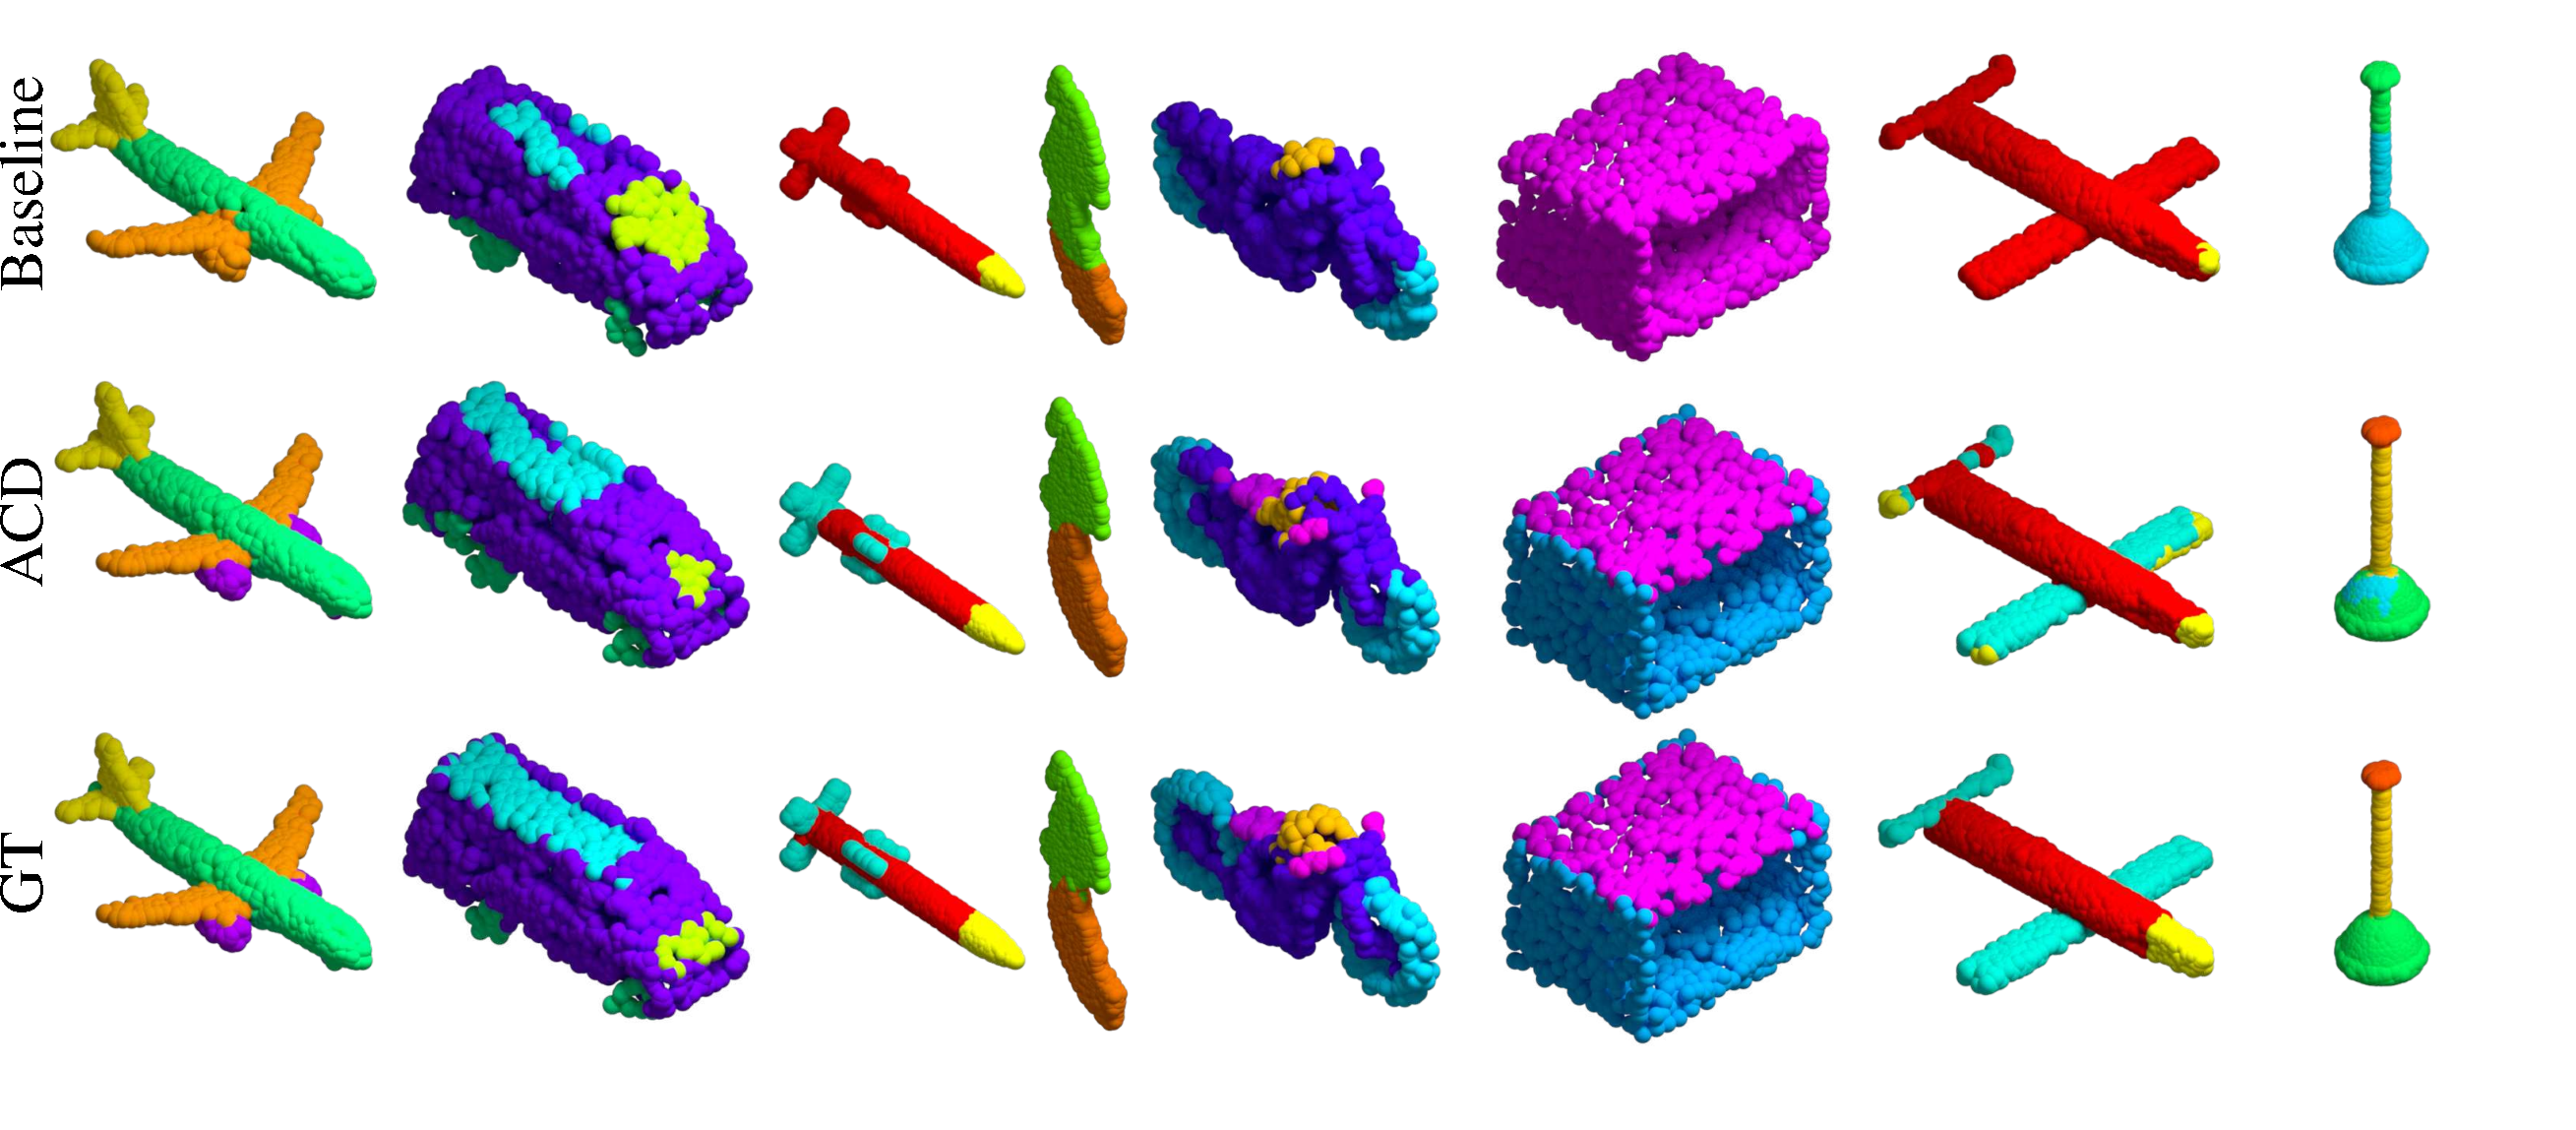
\includegraphics[width=\linewidth]{acd/imgs/segresults_noinput.pdf}
    % \framebox(1\textwidth,200){}
    \caption{\small{Qualitative comparison on 5-shot ShapeNet~\cite{Chang2015ShapeNetAI} part segmentation.
    The baseline method in the first row corresponds to training using only 5 examples per class,
    whereas the ACD results in the second row were computed by performing joint training (cross-entropy from 5 examples + contrastive loss over ACD components from ShapeNetCore).
    The network backbone architecture is the same for both approaches -- PointNet++~\cite{qi2017pointnetpp}.
    The baseline method merges parts that should be separated, \eg engines of the airplane,
    details of the rocket, top of the table, seat of the motorcycle, etc.}}
    \label{fig:segresults}
\end{figure}






% ============================================================
\subsection{Analysis of ACD}
% \todo -- \arc{(i) different backbones - DGCNN and PointNet++ [DONE]; 
% (ii) ACD loss and shape classification performance [DONE]; 
% (iii) concavity tolerance ACD variations and downstream task; 
% (iv) compare decompositions with human parts -- ACD, K-Means, HDBSCAN}


% ------------------------------------------------------------
\noindent
\textbf{On the effect of backbone architectures.}
%
Differently from~\cite{chen2019bae,hassani2019unsupervised,yang2018foldingnet}, the ACD self-supervision does not require any custom network design and should be easily applicable across various backbone architectures. To this end, we use two recent high-performing models -- \textit{PointNet++} (with multi-scale grouping~\cite{qi2017pointnetpp}) and \textit{DGCNN}~\cite{wang2019dynamic} -- as the backbones, reporting results on ModelNet40 shape classification and few-shot segmentation ($k=5$) on ShapeNetSeg (Table~\ref{tab:arch_modelnet}). On shape classification, both networks show large gains from ACD pre-training: 11\% for PointNet++ (as reported earlier) and 14\% for DGCNN.
%
On few-shot segmentation with 5 samples per category (16 shape categories), PointNet++ improves from 68.14\% IoU to 72.3\% with the inclusion of the ACD loss. The baseline DGCNN performance with only 5 labeled samples per class is relatively lower (64.14\%), however with the additional ACD loss on unlabeled samples, the model achieves 73.11\% IoU, which is comparable to the corresponding PointNet++ performance (72.30\%). 

\begin{table}[t]
\centering
\caption{\small{Comparing embeddings from PointNet++~\cite{qi2017pointnetpp} and DGCNN~\cite{wang2019dynamic} backbones: shape classification accuracy on ModelNet40 (\textit{Class./MN40}) and few-shot part segmentation performance in terms of class-averaged IoU on ShapeNet (\textit{Part Seg./ShapeNet}).
}}
\label{tab:arch_modelnet}
\begin{tabular}{@{\extracolsep{6pt}}llcc}
\toprule
\textbf{Task / Dataset}      & \textbf{Method}   & \textbf{PointNet++}  & \textbf{DGCNN} \\
\midrule
\multirow{2}{*}{Class./MN40} & Baseline    & 77.96        &  74.11 \\
                             & w/ ACD  & \textbf{89.06}   &  \textbf{88.21} \\
\midrule
\multirow{2}{*}{5-shot Seg./ShapeNet} & Baseline   & 68.14 $\pm$ 0.90 & 64.14 $\pm$ 1.43 \\
                             & w/ ACD         & \textbf{72.30} $\pm$ 1.80 & \textbf{73.11} $\pm$ 0.95 \\
\bottomrule
\end{tabular}
\end{table}


% ------------------------------------------------------------
\begin{figure}
% \begin{figure}[t]
% \begin{wrapfigure}{R}{0.5\textwidth}
    \centering
    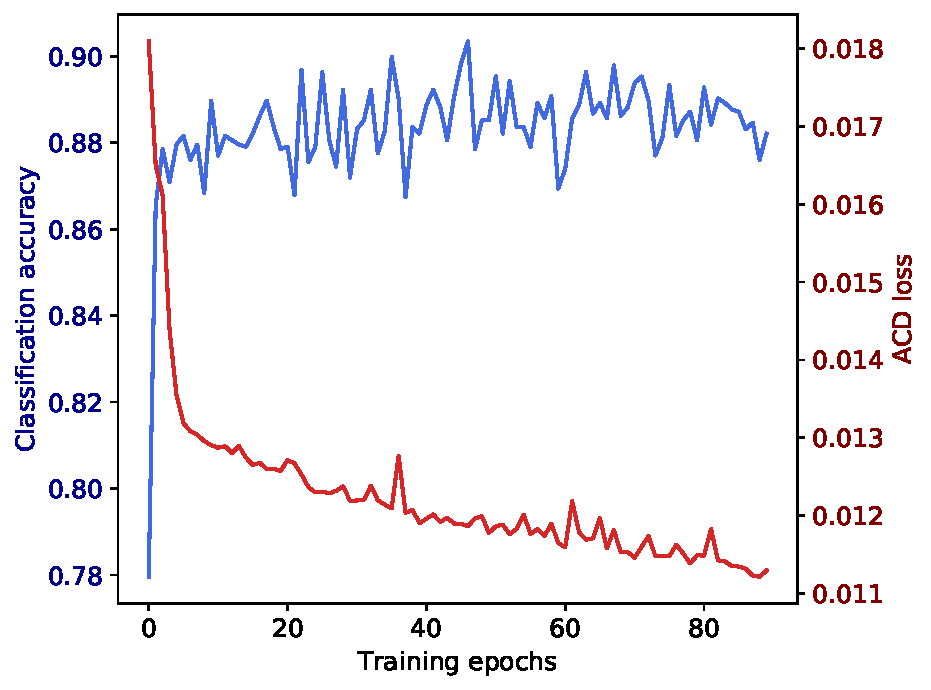
\includegraphics[width=0.6\textwidth]{acd/imgs/train_svm_acd.pdf}
    \caption{\small{Classification accuracy of a linear SVM on the ModelNet40 \emph{validation set} v.s. 
    the ACD \emph{validation loss} over training epochs. 
    % Doing better on ACD also leads to learning representations that are useful for shape classification on ModelNet40.}
    }}
    \vspace{-0.5cm}
    \label{fig:acd_loss_svm}
\end{figure}
\vspace{2mm}
\noindent
\textbf{On the role of ACD in shape classification.} 
Fig.~\ref{fig:acd_loss_svm} shows the reduction in validation loss on learning ACD (red curve) as training progresses on the unlabeled ShapeNet data.  Note that doing well on ACD (in terms of the validation loss) also leads to learning representations that are useful for the downstream tasks of shape classification (in terms of SVM accuracy on a validation subset of ModelNet40 data, shown in blue).


% \end{figure}
%
However, the correlation between the two quantities is not very strong (Pearson $\rho = 0.667$) -- from the plots it appears that after the initial epochs, where we observe a large gain in classification accuracy as well as a large reduction in ACD loss, continuing to be better at the pretext task does not lead to any noticeable gains in the ability to classify shapes: training with ACD gives the model some useful notion of grouping and parts, but it is not intuitively obvious if \textit{perfectly} mimicking ACD will improve representations for classifying point-clouds into shape categories.



% ------------------------------------------------------------
\begin{figure}[t]
    \centering
    \begin{tabular}{@{\extracolsep{1pt}}cccc}
    ACD & K-means & Spectral & HAC \\
    
    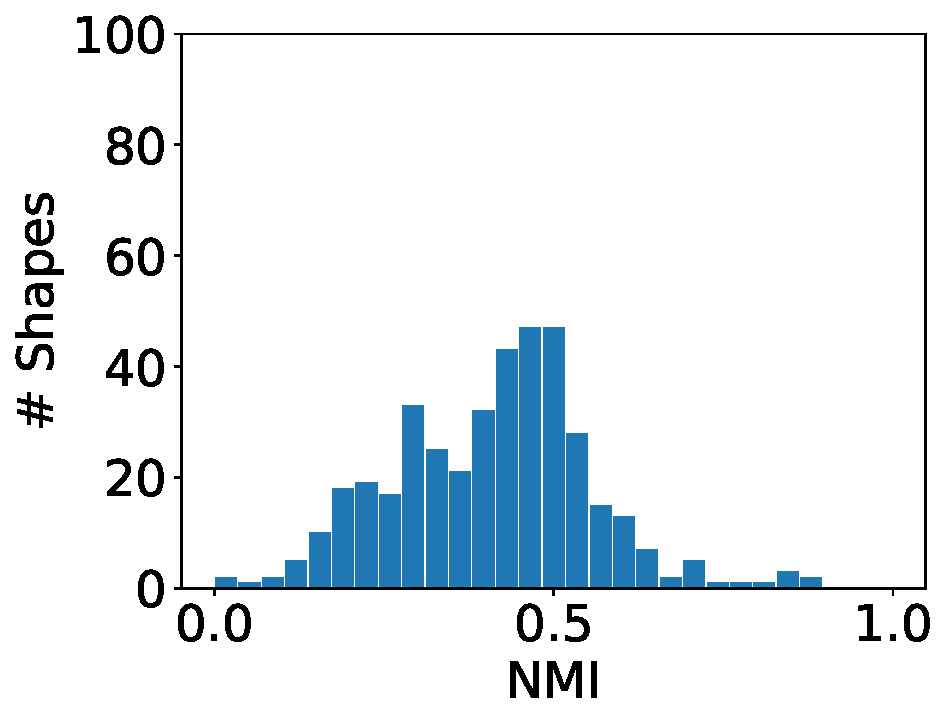
\includegraphics[width=0.2\textwidth]{acd/imgs/acd_nmi_hist.pdf} &
    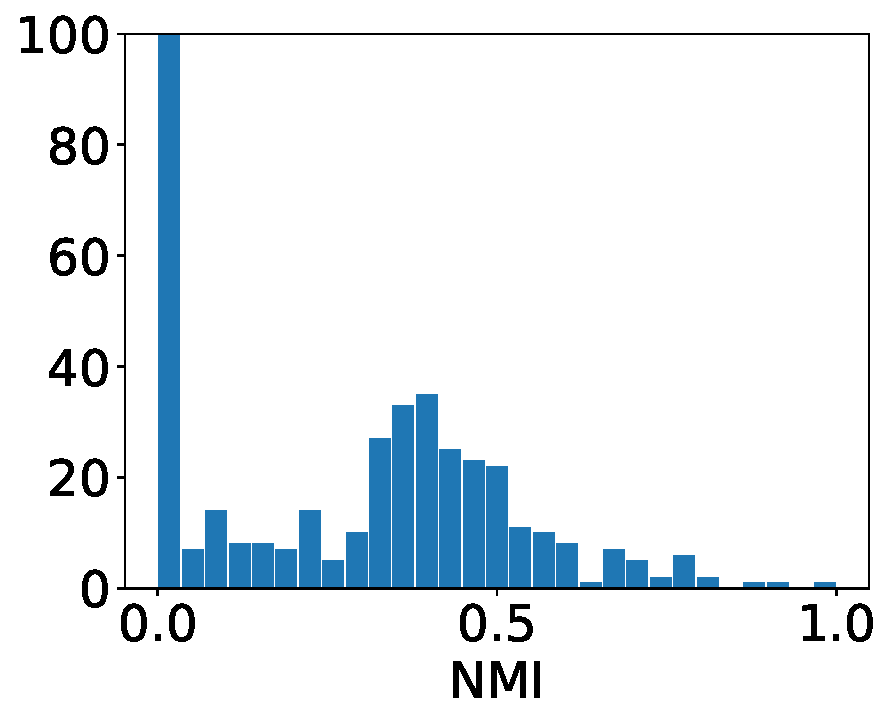
\includegraphics[width=0.2\textwidth]{acd/imgs/kmeans_nmi_hist.pdf} & 
    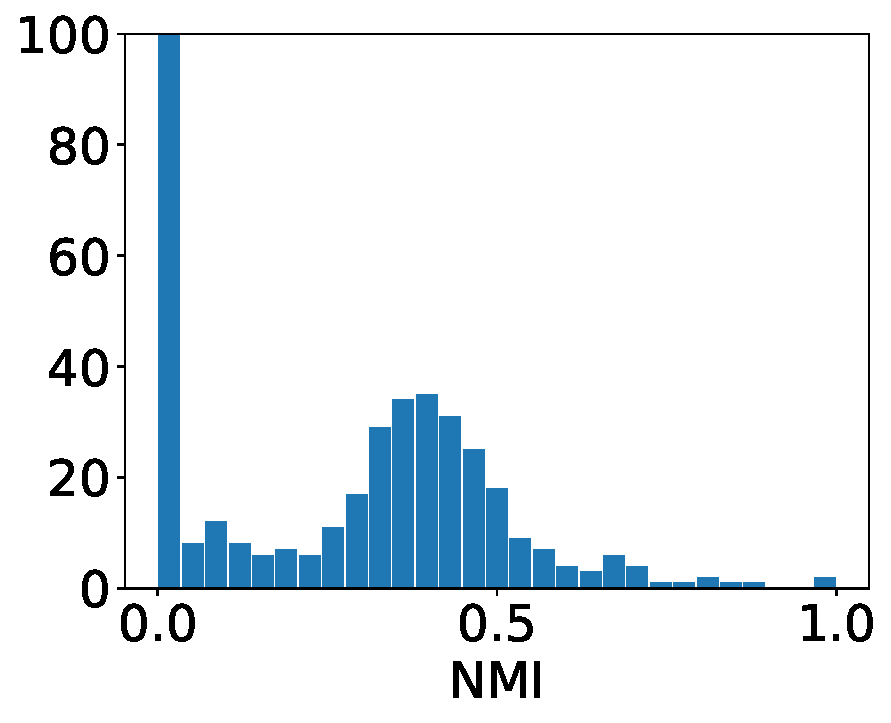
\includegraphics[width=0.2\textwidth]{acd/imgs/spectral_nmi_hist.pdf} & 
    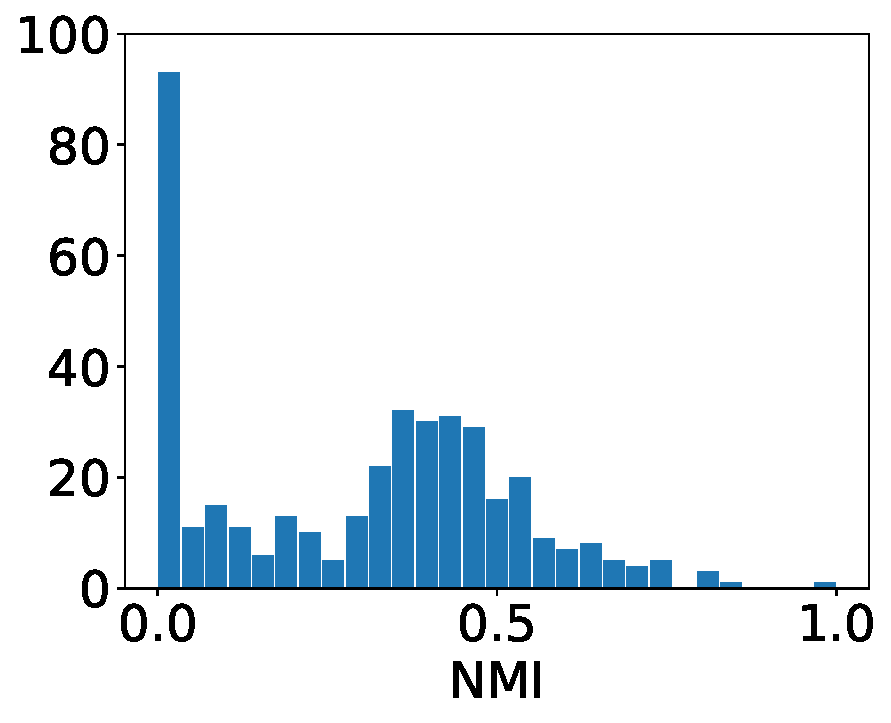
\includegraphics[width=0.2\textwidth]{acd/imgs/hac_nmi_hist.pdf} \\
    \hspace{0.1cm}
    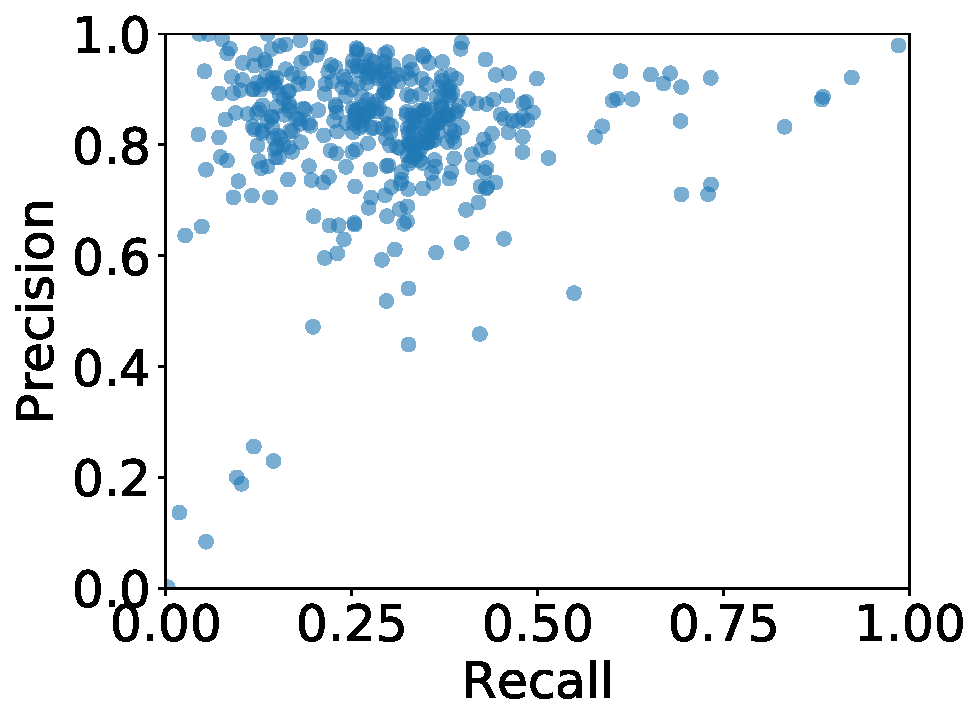
\includegraphics[width=0.2\textwidth]{acd/imgs/acd_pr.pdf} &
    \hspace{0.1cm}
    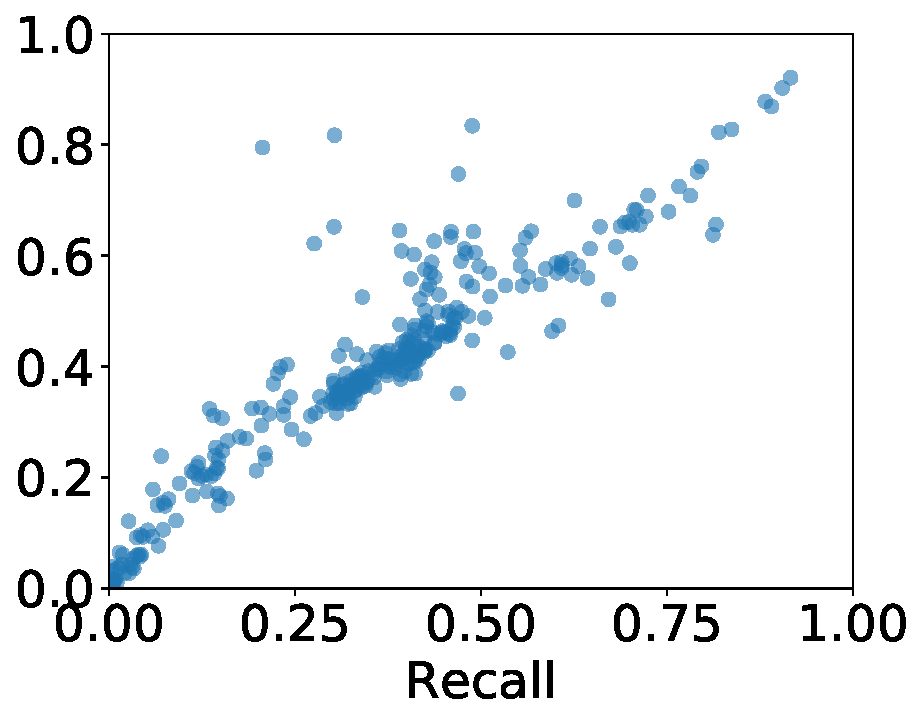
\includegraphics[width=0.2\textwidth]{acd/imgs/kmeans_pr.pdf} &
    \hspace{0.1cm}
    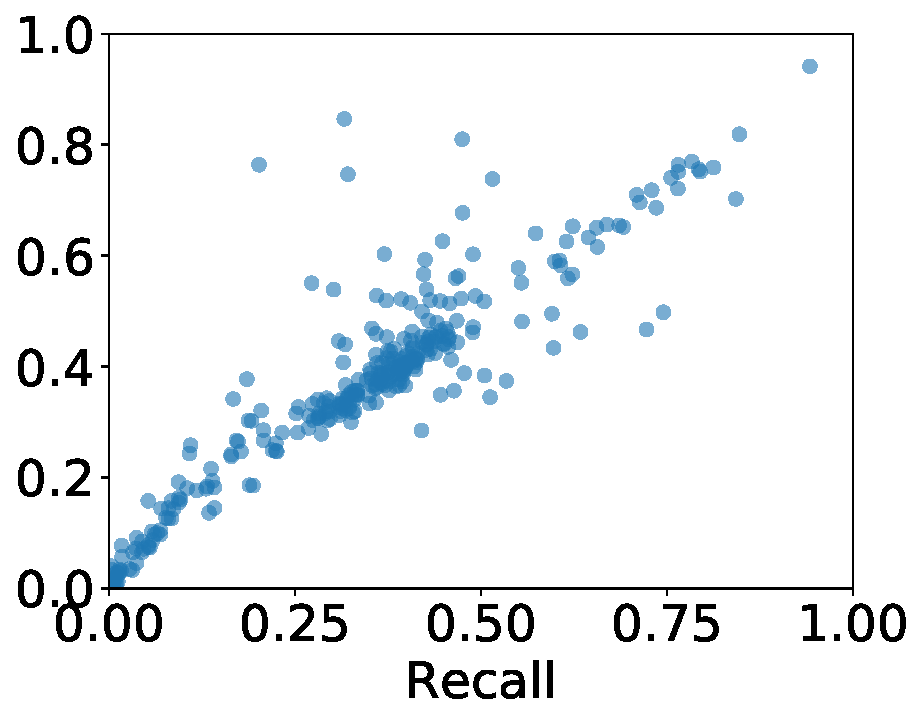
\includegraphics[width=0.2\textwidth]{acd/imgs/spectral_pr.pdf} &
    \hspace{0.1cm}
    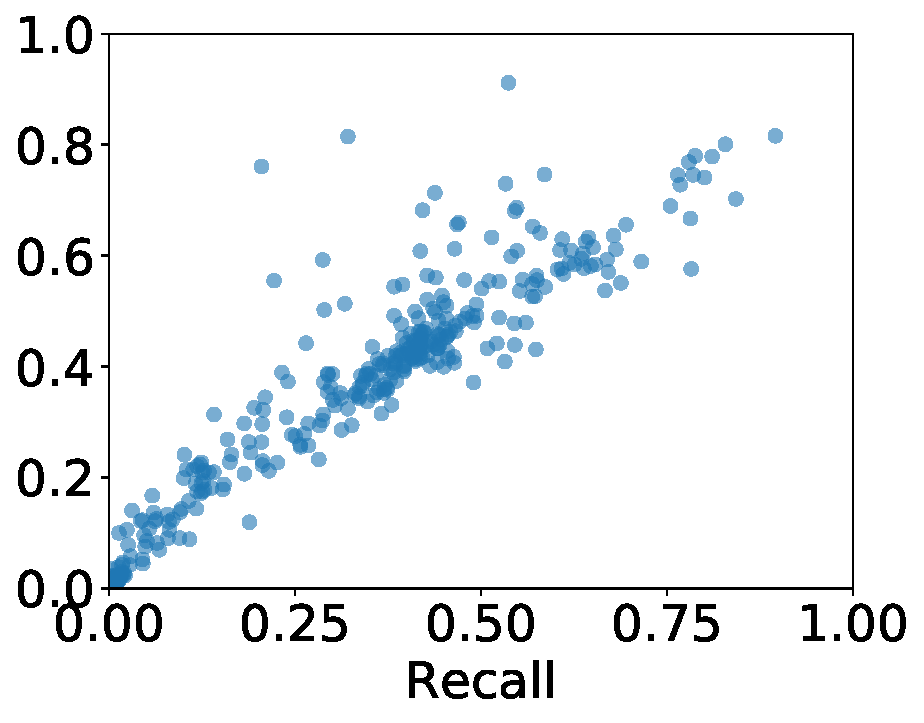
\includegraphics[width=0.2\textwidth]{acd/imgs/hac_pr.pdf} \\
    % \framebox(\textwidth,90pt){}
    % \emptybox{90pt}
    \end{tabular}
    \caption{ \small{Correspondence between human part labels and shape decompositions: comparing ACD with basic clustering algorithms -- K-means, spectral clustering and hierarchical agglomerative clustering (HAC). \textbf{\textit{Row-1:}} histogram of \textit{normalized mutual information} (NMI) between human labels and clustering -- ACD is closer to the ground-truth parts than others (y-axes clipped at 100 for clarity). 
    \textbf{\textit{Row-2:}} plotting \textit{precision v.s. recall} for each input shape, ACD has high precision and moderate recall (tendency to over-segment parts), while other methods are usually lower in both metrics.}}
    \label{fig:acd_nmi}
\end{figure}

% ------------------------------------------------------------
\vspace{2mm}
\noindent
\textbf{Comparison with clustering algorithms.}
We quantitatively analyse the connection between convex decompositions and semantic object parts  by
comparing ACD with human part annotations on 400 shapes from ShapeNet, along with simple clustering baselines -- K-means~\cite{arthur2006k}, spectral clustering~\cite{shi2000normalized,von2007tutorial} 
and hierarchical agglomerative clustering (HAC)~\cite{mullner2013fastcluster} on $(x,y,z)$ coordinates 
of the point clouds. For the baselines, we set the number of clusters to be the number of ground-truth
parts in each shape. 
%
For each sample shape, given the set of $M$ part categories $\Omega = \{ \omega_1, \omega_2, \dots \omega_M \}$ 
and the set of $N$ clusters $\mathcal{C} = \{ C_1, C_2, \dots C_N  \}$, clustering performance is 
evaluated using \textit{normalized mutual information} (NMI)~\cite{vinh2010information}, defined as 
%
\begin{equation}
    \text{NMI}(\Omega, \mathcal{C}) = \frac{I(\Omega; \mathcal{C})}{ [H(\Omega) + H(\mathcal{C})]/ 2},
\end{equation}
%
where $I(\cdot ; \cdot)$ denotes the mutual information between classes $\Omega$ and clusters $\mathcal{C}$,
and $H(\cdot)$ is the entropy~\cite{cover2012elements}. A better clustering results in \textit{higher} NMI 
w.r.t. the ground-truth part labels. 
%
The first row of Fig.~\ref{fig:acd_nmi} shows the histograms of NMI between cluster assignments and human 
part annotations: ACD, though not
exactly aligned to human notions of parts, is significantly better than other clustering methods, which
have very low NMI in most cases. 

We plot the \textit{precision} and \textit{recall} of clustering for each of the 400 shapes on the second row of
Fig.~\ref{fig:acd_nmi}. 
The other baseline methods show that a na\"ive clustering of points does not correspond well to semantic
parts. 
% \footnote{We note that more sophisticated shape decomposition baselines do exist, however our goal is to demonstrate the motivation behind using ACD v.s. simpler algorithms.}
ACD has high precision and moderate recall on most of the shapes -- this agrees with the visual impression
that though ACD tends to oversegment the shapes, the decompositions contain most of the boundaries present
in the human annotations.
For example, ACD typically segments the legs of a chair into four separate components. Part annotations on
ShapeNet however label all the legs of a chair with the same label, since the benchmark does not
distinguish between the individual legs of a chair.
We note that the correspondence of ACD to human part labels is not perfect, and this opens an interesting
avenue for further work -- exploring other decomposition methods like generalized cylinders~\cite{gdc}
that may correspond more closely to human-defined parts, and in turn could lead to improved downstream
performance on discriminative tasks.



